\section{Umsetzung in TwinCAT} \label{Skillumsetzung in TwinCAT}

	\subsection{Allgemeine Struktur} \label{Skill_Allgemeine Struktur}
		 \begin{wrapfigure}{r}{0.5\textwidth}
			\centering
			\includegraphics[width=0.5\textwidth]{06_Skillentwicklung/UmsetzungsstrukturSkill}
			\captionsetup{justification=centering}
			\caption{Umsetzungsstruktur}
			\label{fig:Umsetzungsstruktur_Skill}
		\end{wrapfigure} \par
		Die Programmierung der Skills soll einfach und übersichtlich gehalten werden. Dafür wird mit den bereits angesprochenen Interfaces gearbeitet, aber auch mit Vererbungen von Funktionsbausteinen (\ref{fig:Umsetzungsstruktur_Skill}). Über eine Vererbung können Methoden und Eigenschaften (inkl. Ihrer Funktionalität), sowie Variablendeklaration von einem Funktionsbaustein übernommen werden. Dadurch kann ein Basis-Funktionsbaustein erstellt werden, welcher Methoden, Eigenschaften und Variablen zur Verfügung stellt, welche für alle Skills verwendet werden. Diese Elemente werden bei jeder Vererbung separat zur Verfügung gestellt. Mehrere Skills greifen nicht auf die selben Elementen zu und beeinflussen sich somit nicht. 
		\\
		Da jedoch die Steuerungselemente auf das instanziierte Objekt zugreifen sollen (Skizze), können diese nicht in einem Basis-Funktionsblock abgebildet und vererbt werden. Für die Objekte gibt es verschiedene Interfaces, je nach benötigten Daten für den Prozess. Entsprechend werden in unterschiedlichen Skills auch unterschiedliche Objekt-Interfaces benötigt. Dadurch kann das Objekt nicht bereits im Basis-Funktionsbaustein instanziiert werden und die Methoden und Eigenschaften können nicht darauf zugreifen. Aus diesem Grund, müssen «\verb|M_Start|», «\verb|M_Stop|», «\verb|M_Reset|» und «\verb|P_State|» im Skill selber implementiert werden. Die Vererbung wird in diesem Fall nur für Variablen genutzt, welche für alle Skills gleich bleiben.
		\\
		In TwinCAT wird eine Vererbung über den Zusatz «\verb|EXTENDS|» durchgeführt. Ein Interface kann mit dem Zusatz «\verb|IMPLEMENTS|» zugewiesen werden. 
		\\
		Für den Basis-Funktionsbaustein «\verb|FB_Basis_Skill|» wurden die Variablen wie folgt definiert: 
		
		\begin{figure}[h!]
			\centering
			\fbox{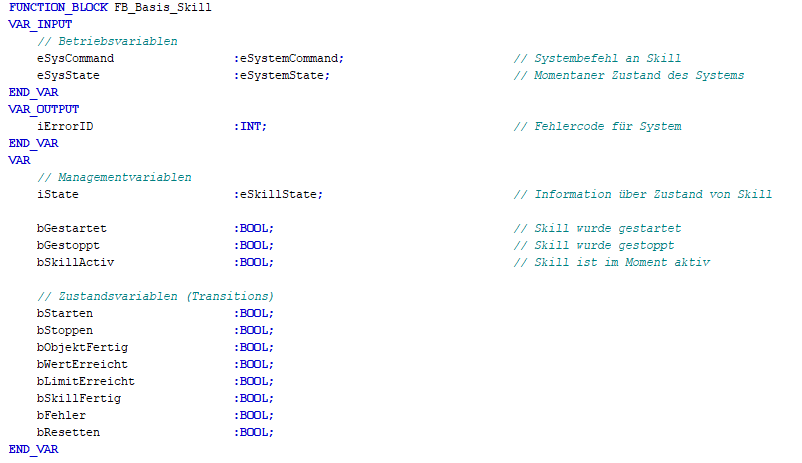
\includegraphics[width=0.8\textwidth]{06_Skillentwicklung/FB_Basis_Skill}}
			\captionsetup{justification=centering}
			\caption{Definitionen für Skill-Basis-FB}
			\label{fig:FB_Basis_Skill}
		\end{figure}
	
	\subsection{Aufbau des Grund-Skills} \label{Grundskill_Aufbau}
		Alle Skills sollten nach einem einheitlichen Grundmuster aufgebaut werden. Dabei wird ein Skill als Funktionsblock mit strukturiertem Text realisiert. Die Verwendung von strukturiertem Text bietet hohe Flexibilität bei der Umsetzung.
		\\
		\\
		Jeder Skill hat folgende drei Steuerungsmethoden: 
		\begin{figure}[h!]
			\centering
			\begin{subfigure}[b]{0.5\textwidth}
				\centering
				\fbox{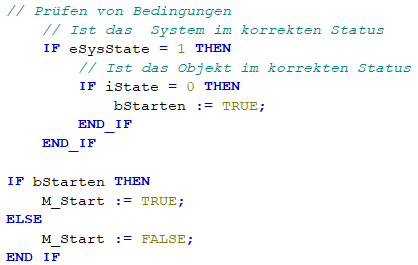
\includegraphics[width=\textwidth]{06_Skillentwicklung/MStart}}
				\caption{Methode: Start}
				\label{fig:Skill_MStart}
			\end{subfigure}
			\hfill
			\begin{subfigure}[b]{0.2\textwidth}
				\centering
				\fbox{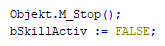
\includegraphics[width=\textwidth]{06_Skillentwicklung/MStop}}
				\caption{Methode: Stop}
				\label{fig:Skill_MStop}
			\end{subfigure}
			\hfill
			\begin{subfigure}[b]{0.2\textwidth}
				\centering
				\fbox{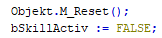
\includegraphics[width=\textwidth]{06_Skillentwicklung/MReset}}
				\caption{Methode: Reset}
				\label{fig:Skill_MReset}
			\end{subfigure}
			\caption{Steuerungsmethoden eines Skills}
			\label{fig:Steuerungsmethoden}
		\end{figure}
		
		Innerhalb der Methode \verb|M_Start| (\ref{fig:Skill_MStart}) wird in einem ersten Schritt geprüft, ob sich das System im korrekten Zustand befindet. Danach wird der Zustand des Skills geprüft. Da die Methode von aussen (zum Beispiel durch die Sequenz) ausgelöst wird, darf der Skill nur im BEREIT-Zustand bestartet werden. Als letzter Schritt werden die Parameter überprüft, falls diese Auflagen erfüllen müssen. Falls alle Bedingungen erfüllt werden, werden die Prozessparameter (in diesem Fall wird eine Roboterposition) übergeben und die Start-Methode des Objektes wird ausgelöst. Die Stop- und Reset-Methode lösen die entsprechenden Methoden beim Objekt aus (\ref{fig:Skill_MStop} / \ref{fig:Skill_MReset}).
		\\
		Der Aufbau eines Skills gliedert sich in drei Hauptbereiche: Fehlerüberwachung, Aufruf interner Steuerungsmethoden und Zustandsmanagement. Im Bereich des Aufrufs interner Steuerungsmethoden wird überprüft, ob das System vorgibt, den Skill zu stoppen oder zurückzusetzen (\ref{fig:Methodenaufruf}). In diesen Fällen wird entweder die Methode \verb|M_Stop| oder \verb|M_Reset| ausgelöst. Zudem wird geprüft, ob der Skill ein definiertes Limit oder einen Zielwert erreicht. Auch hier führt dies zur Ausführung der Methode \verb|M_Stop|.
		
		\begin{figure}[h!]
			\centering
			\fbox{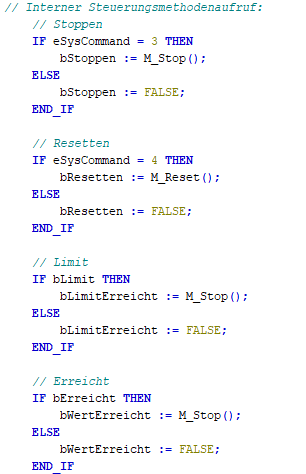
\includegraphics[width=0.26\textwidth]{06_Skillentwicklung/Methodenaufruf}}
			\captionsetup{justification=centering}
			\caption{Interner Steuerungsmethodenaufruf}
			\label{fig:Methodenaufruf}
		\end{figure}
		
		\newpage
		
		Unter Zustandsmanagement werden die, in Kapitel \ref{Softwareinteraktion} definierten Zustände des Skills definiert und umgesetzt. Für die Umsetzung wurde mit einer CASE-Anwendung gearbeitet.  Die meisten Zustände sind für alle Skills identisch, jedoch beim Zustand «LAUFEND» gibt es kleinere Unterschiede. 
		
		\begin{tabularx}{\textwidth}{@{}>{}p{13em} X@{}}
			Zustand 0 - BEREIT: & 
			Innerhalb des Zustandes prüft der Skill den Zustand des Objektes. Falls das Objekt durch \verb|M_Start| gestartet wurde und sich nun im Zustand LAUFEND befindet, so wechselt auch der Skill auf den Zustand  LAUFEND. Der Skill darf jedoch nur dann auf  den Objektzustand reagieren, falls der Skill den Start des Objektes auch ausgelöst hat, da unter Umständen mehrere Skills auf ein Objekt zugreifen. 
			\\
			Zustand 1 - LAUFEND: & 
			Der Skill kann auf verschiedene Arten gestoppt werden, welche innerhalb des Zustandes überprüft werden. Das System kann den Skill stoppen, welcher anschliessend direkt in den Zustand BEREIT wechselt. Falls der Objektzustand meldet, dass das Objekt den Prozess abgeschlossen hat (zum Beispiel bei einer Punkt-zu-Punkt-Bewegung eines Roboters), wechselt der Skill in den Zustand ABGESCHLOSSEN. Falls eine Limit- oder Erreicht-Bedingung erfüllt wurde, wird das Objekt durch den Skill gestoppt und wechselt in den entsprechenden Zustand. Während der Zustands LAUFEND können aber auch interne Methoden aufgerufen werden (zum Beispiel für das Auswerten von Messwerten).
			\\
			Zustand 2 - ABGESCHLOSSEN: & 
			Der Zustand gibt den Befehl zum Resetten an das Objekt weiter. Sobald der Objektzustand meldet, dass sich das Objekt im Zustand BEREIT befindet, kehrt auch der Skill in den Zustand BEREIT zurück. 
			\\
			Zustand 3 - FEHLER: & 
			Im Fehlerzustand wartet der Skill, dass dieser durch das System resettet wird. 
			\\
			Zustand 4 - LIMIT: & 
			Der Zustand gibt den Befehl zum Resetten an das Objekt weiter. Sobald der Objektzustand meldet, dass sich das Objekt im Zustand BEREIT befindet, kehrt auch der Skill in den Zustand BEREIT zurück.
			\\
			Zustand 5 - ERREICHT: & 
			Der Zustand gibt den Befehl zum Resetten an das Objekt weiter. Sobald der Objektzustand meldet, dass sich das Objekt im Zustand BEREIT befindet, kehrt auch der Skill in den Zustand BEREIT zurück.
			\\
		\end{tabularx}
		
		\newpage
	
	\subsection{Erarbeitete Skills} \label{Skills_Erarbeitet}
		Zum Stand der Dokumentation wurden drei Skills umgesetzt, welche sich auf den Roboter (2 Skills) und den Greifer (1 Skill) beziehen. 	
		
		\begin{bfhNoteBox}
			Aus Zeitgründen wurde während der Erarbeitung entschieden, dass das Kamerasystem noch nicht in den Prozess integriert wird. Der Schwerpunkt dieser Arbeit liegt auf der Software-Struktur und wie die verschiedenen Elemente miteinander interagieren. Auch ohne Kamerasystem konnte die Struktur definiert, aufgebaut und getestet werden. Die Einarbeitung in das Vision-Tool von TwinCAT ist ein zeitintensiver Prozess, mit wenig Mehrwert für das Ziel dieser Arbeit. Im Rahmen einer weiterführender Arbeit, wäre die Integration des Kamerasystem aber ein relevanter Punkt. 
		\end{bfhNoteBox}
		\vspace{3mm}
		
		\textbf{Skill 1 (Roboter):} \verb|Skill_Position_Anfahren|
		\vspace{2mm} 
		\\
		Mit dem Skill kann eine Position vom Roboter angefahren werden. Die Bewegung wird selbständig vom Objekt abgeschlossen. Es ist nicht vorgesehen, dass der Skill die Bewegung stoppt. Damit der Skill ausgeführt werden kann, benötigt er folgende Prozessparameter, welche als Eigenschaften (SET) dem Skill übergeben werden: 
		
		\newcolumntype{L}[1]{>{\raggedright\let\newline\\\arraybackslash\hspace{0pt}}m{#1}}
		\begin{table}[ht]
			\centering
			\colorlet{BFH-table}{BFH-MediumBlue!10}
			\colorlet{BFH-tablehead}{BFH-MediumBlue!50}
			\begin{bfhTabular}{| l | L{3.5cm} | L{6.5cm} |}
				Bezeichnung: 				& Typ:					& Beschreibung:									
				\\\hline
				\verb|P_RobotPosition|		& Array[0..5] of LREAL	& Gibt die kartesischen Koordinaten oder Gelenkwinkel an, je nachdem welcher Bewegungstyp ausgewählt wurde.			
				\\\hline
				\verb|P_RobotSpeed |		& LREAL					& Gibt an, wie schnell sich der Roboter bewegen soll.		
				\\\hline
				\verb|P_RobotAcceleration|	& LREAL					& Gibt an, mit welcher Beschleunigung der Roboter arbeiten soll.		
				\\\hline
				\verb|P_RobotMoveTyp|		& eRobPosTyp			& Gibt den Bewegungstyp des Roboters an.
				\\\hline
				\verb|P_RobotPosTyp|		& eRobMoveTyp			& Gibt den Positionstyp der angegebenen Position an.				
			\end{bfhTabular}
			\caption{Skill 1: Eigenschaften}
			\label{tab:Skill_1_Eigenschaften}
		\end{table}
		
		Für den Bewegungstyp und Positionstyp wurden benutzerdefinierte Listen-Datentypen angelegt. Eine detaillierte Erklärung ist bei der Beschreibung des Roboter-Objektes (Kapitel \ref{Objekt_Erarbeitet}) vorhanden. Diese sind wie folgt definiert: 
		
		 \begin{table}[ht]
			\centering
			\colorlet{BFH-table}{BFH-MediumBlue!10}
			\colorlet{BFH-tablehead}{BFH-MediumBlue!50}
			\begin{bfhTabular}{ccc}
				Listen-Nr: 	& eRobPosTyp:	& eRobMoveTyp:									
				\\\hline
				0			& Absolut		& LinearToolSpace				
				\\\hline
				1			& Relativ 		& LinearJointSpace				
				\\\hline
				2			& /				& CircularToolSpace			
				\\\hline
				3			& /				& BlendCircularMoveLinear			
			\end{bfhTabular}
			\captionsetup{justification=centering}
			\caption{Benutzerdefinierte Datentypen für Roboter}
			\label{tab:Datentypen_Benutzerdefiniert_Roboter}
		\end{table}
		\newpage
		
		\textbf{Skill 2 (Roboter):} \verb|Skill_Position_Anfahren_Erweitert|
		\vspace{2mm} 
		\\
		Ist ähnlich wie Skill 1, jedoch kann der Skill noch auf eine Kraft reagieren. Es ist möglich einen Grenzwert für die Kraft und deren Richtung anzugeben. Der Skill stoppt das Objekt und somit die Bewegung, falls dieser Grenzwert überschritten wurde. Damit ist es möglich Hindernisse zu erkennen, um zum Beispiel einen Anschlag zu definieren. Damit der Skill ausgeführt werden kann, werden die Eigenschaften von Skill 1 mit folgender Eigenschaft ergänzt:
		
		\newcolumntype{L}[1]{>{\raggedright\let\newline\\\arraybackslash\hspace{0pt}}m{#1}}
		\begin{table}[ht]
			\centering
			\colorlet{BFH-table}{BFH-MediumBlue!10}
			\colorlet{BFH-tablehead}{BFH-MediumBlue!50}
			\begin{bfhTabular}{| l | L{3.5cm} | L{7.5cm} |}
				Bezeichnung: 				& Typ:					& Beschreibung:									
				\\\hline
				\verb|P_Erreicht|			& sKraftvariablen		& Gibt den Grenzwert für die entsprechenden Richtungen an.				
			\end{bfhTabular}
			\caption{Skill 2: Eigenschaften}
			\label{tab:Skill_2_Eigenschaften}
		\end{table}
		
		Der Datentyp "\verb|sKraftvariablen|" ist eine Struktur, welche drei LREAL-Elemente besitzt. Diese stellen die Kraft in X-, Y- und Z-Richtung dar. 
		
		\textbf{Skill 3 (Greifer):} \verb|Skill_GreiferPos_Anfahren|
		\vspace{2mm} 
		\\
		Der letzte Skill bezieht sich auf den Greifer. Der Skill kann in Verbindung mit einem Greifer wegwendet werden, welche eine definierte Position anfahren kann. Die Bewegung wird selbständig vom Objekt abgeschlossen. Damit der Skill ausgeführt werden kann, benötigt er folgende Prozessparameter, welche als Eigenschaften (SET) dem Skill übergeben werden: 
		
		\newcolumntype{L}[1]{>{\raggedright\let\newline\\\arraybackslash\hspace{0pt}}m{#1}}
		\begin{table}[ht]
			\centering
			\colorlet{BFH-table}{BFH-MediumBlue!10}
			\colorlet{BFH-tablehead}{BFH-MediumBlue!50}
			\begin{bfhTabular}{| l | L{1.5cm} | L{8cm} |}
				Bezeichnung: 					& Typ:			& Beschreibung:									
				\\\hline
				\verb|P_GreifBreite|			& LREAL		& Gibt an, welche Breite die Greifbacken anfahren sollen.		
				\\\hline
				\verb|P_GreifGeschwindigkeit|	& LREAL			& Gibt an, wie schnell sich die Greifbacken bewegen sollen.		
				\\\hline
				\verb|P_GreifKraft|				& LREAL			& Gibt an, mit welcher Kraft die Greifbacken zudrücken sollen.
			\end{bfhTabular}
			\caption{Skill 3: Eigenschaften}
			\label{tab:Skill_3_Eigenschaften}
		\end{table}
		
	\subsection{Momentaner Stand} \label{Skill_Momentaner_Stand}
	Die Skills wurden derzeit so entwickelt, dass die definierte Anwendung erfolgreich umgesetzt werden kann. Dabei lag der Fokus nicht darauf, bereits jede mögliche Situation abzudecken. Viel Zeit und Aufwand wurden in die Konzeption und das Testen der Skill-Struktur investiert. Diese Struktur bildet das stabile und zuverlässige Fundament, auf dem die Skills aufbauen. Sobald dieses Fundament steht, können die Funktionen des Skills schrittweise erweitert und optimiert werden.
	\\
	Als potenzielle Erweiterung könnten zusätzliche Einstellungsmöglichkeiten integriert werden. Beim Greifer könnte beispielsweise ein Offset angegeben werden, der die Dicke der Backenaufsätze berücksichtigt. Dadurch ließe sich die angefahrene Breite der Greifbacken an unterschiedliche Aufsätze anpassen.
	
	